\section{Extensible Data Import Framework}\label{sec:import-framework}

\textbf{Authorship}
\vspace*{4mm}

\begin{longtable}{@{}llll@{}}
\toprule
Version & Date & Modified by & Summary of changes \\
\midrule
\endhead
0.1 & 2017-07-20 & Rohullah, Jawid & Initial version \\
0.1a & 2017-07-21 & Rohullah, Jawid & framework description \\
0.1b & 2017-07-22 & Rohullah, Jawid & evaluations, features, improvements, values parts \\
0.2 & 2017-07-26 & Andres & Proofread: spelling, readability, etc. \\
0.2a & 2017-07-28 & Andres & Further refinement of text \\
0.3 & 2017-07-28 & Rohullah, Jawid & framework structure explanations + diagrams \\
\bottomrule
\end{longtable}

\vspace*{4mm}

The Open Data Platform which we have built for extracting, transforming
and loading open sensor data is made up several significant components
to efficiently process the large quantity of incoming data.

The first part of the system requires a powerful tool to do the job of
importing very large amounts of different kinds of data with various
formats and types from several data sources in a performant manner.

The job of the importers, in addition to fetching data from its source,
is mainly to apply a series of rules and transformations to the source
data in order to fit the our schema and be stored in the system.

For this purpose, a framework that supports the entire processes of
extracting and transforming data is desirable.

In addition to the main import functionality, additional requirements
and criteria were considered regarding the framework.

This chapter describes the requirements, selection criteria, design
decisions, evaluations, technical implementation details, further
possible improvements, as well as the value of having such a framework.

\subsection{Framework Requirements}\label{framework-requirements}

The following are use-cases which our framework should cover:

\begin{itemize}
\tightlist
\item
  user can add a new data source with minimal coding and configuration
  effort.
\item
  provide various functionalities to the user such as processing data
  into customized format/schema
\item
  reusable components for reading, processing and writing data.
\item
  ideally the framework may be provided as a starter application which
  doesn't require it be built from scratch every time.
\item
  the framework should support extracting data from known transport
  channels and in known formats.
\item
  the entire framework must be based on microservices architecture (as
  opposed to a monolithic system).
\item
  the framework should include logging functionalities.
\item
  if an importer were to crash while importing data, it should continue
  from the point where it failed after being restarted.
\end{itemize}

\subsection{Evaluation of different data import
frameworks}\label{evaluation-of-different-data-import-frameworks}

According to the framework requirements, we needed to search and find a
useful and powerful tool such as an existing ETL framework or a
technology on top of which we could build our data import framework.
Therefore, it seemed to be a good idea to compare these frameworks and
come up with the best decision. So we compared a couple of existing
frameworks and technologies with different aspects such as:

\begin{itemize}
\tightlist
\item
  Functional and non-functional aspects of different frameworks are
  considered.
\item
  Popularity of its programming language
\item
  Popularity of its user community
\item
  Open source or open license
\item
  Capable of being deployed as a microservice to the Cloud
\item
  Capable of scheduling the jobs
\item
  Processing of jobs into batches
\item
  Recoverability of individual jobs from failures
\end{itemize}

\subsubsection{Evaluated Existing
Frameworks}\label{evaluated-existing-frameworks}

\begin{enumerate}
\def\labelenumi{\arabic{enumi}.}
\tightlist
\item
  Spring Batch

  \begin{itemize}
  \tightlist
  \item
    Spring Cloud Tasks
  \item
    Spring Cloud Data Flow
  \end{itemize}
\item
  Java EE
\item
  Easy Batch
\item
  Summer Batch
\item
  Talend ETL
\end{enumerate}

\subsection{Design Decisions}\label{design-decisions}

After evaluation and comparison, it was decided to implement our
extensible framework using \textbf{Spring Batch} given the features and
functionality it offers.

\subsubsection{Why Spring Batch}\label{why-spring-batch}

\begin{itemize}
\tightlist
\item
  Lightweight, ready-to-use framework for robust batch processing
\item
  Suitable framework for data integration and processing
\item
  Popular with a large community of users
\item
  Written in a popular language (Java)
\item
  Its \emph{Cloud Task} feature allows the deployment of data importers
  as microservices
\item
  Capabilities for scheduling the jobs in data processing pipeline
\item
  Familiarity to some team members
\end{itemize}

\subsubsection{Spring Batch Features}\label{spring-batch-features}

\begin{enumerate}
\def\labelenumi{\arabic{enumi}.}
\tightlist
\item
  Reusable architecture framework
\item
  Lightweight, enterprise and batch job processing
\item
  Open Source
\item
  Reusable functions such as:

  \begin{itemize}
  \tightlist
  \item
    logging/tracing
  \item
    job processing statistics
  \item
    job restart
  \item
    transaction management
  \end{itemize}
\item
  Concurrent batch processing: parallel processing of a job
\item
  Manual or scheduled restart after failure
\item
  Deployment model, with the architecture JARs, built using Maven.
\item
  The ability to stop/start/restart jobs and maintain state between
  executions.
\end{enumerate}

\subsection{Framework Structure}\label{framework-structure}

Figure \ref{fig:importer-app} shows an abstract overview of a simple importer
application. We will look at each component individually.

\begin{figure}
\centering
	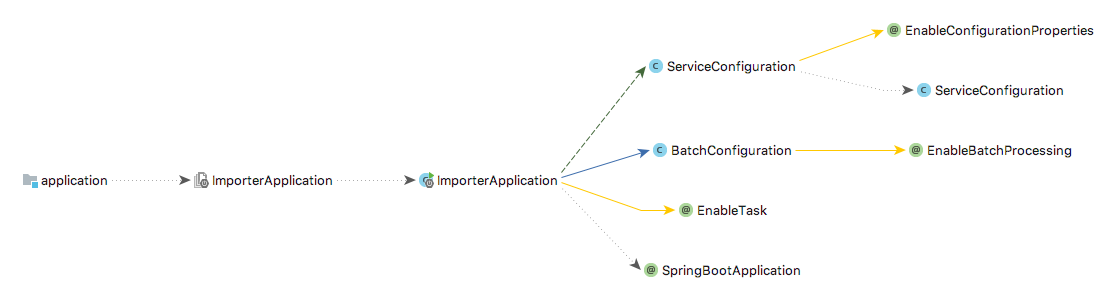
\includegraphics[width=1.00\textwidth]{images/components_diagram.png}
	\caption{Importer Application Overview}
	\label{fig:importer-app}
\end{figure}

\begin{itemize}
\tightlist
\item
  \textbf{ImporterApplication:} Entry point of the importer (Java main
  class).
\item
  \textbf{BatchConfiguration:} Includes configurations on how to read,
  process and write items. It also includes listeners, batch jobs and
  job steps.
\item
  \textbf{Listeners:} Are defined for tracking jobs and steps and
  logging the process of importing to the console.
\item
  \textbf{Jobs:} Generally there is one batch job for each importer. A batch job may have one or more steps for importing a single source.

	\begin{itemize}
		\item \textbf{Steps:} Each step includes a reader, processor, and a writer.

		\begin{itemize}
			\item \textbf{Reader:} Defines how to read items from the source.
			\item \textbf{Processor:} Processes every item - an item is basically an object that represents an record - individually and creates a JSON string for that according to our defined schema.
			\item \textbf{Writer:} Simply writes to Kafka queue.
		\end{itemize}

	\end{itemize}

\item
  \texttt{@SpringBootApplication}: Annotation to make the application a
  Spring Boot Application.
\item
  \texttt{@EnableBatchProcessing}: Annotation to add the functionality
  of processing batch jobs.
\item
  \texttt{@EnableTask}: Enables the deployment of data importers as
  microservices which shutdown once importing is finished.
\item
  \textbf{ServiceConfiguration:} Is the component where the services are
  registered as Java Beans for re-usability. It is included in module
  `library' where re-usable classes across all importers are defined.
  The following other components are included in the `library' module.

	\begin{itemize}
		\item \textbf{ApplicationService:} Includes some generally used methods to bring facility for importing.
		\item \textbf{JsonItemWriter:} Asks \texttt{KafkaRecordProducer} to write individual JSON objects to Kafka queue.
		\item \textbf{KafkaRecordProducer:} Is the class where the items are written to Kafka queue.
		\item \textbf{Schema:} Each importer should have at least one model class which has all the necessary fields for reading records from a source; all these classes are extended from Schema.
		\item \textbf{JsonStringBuilder:} The class which contains functions for creating a json string according to our defined schema.
	\end{itemize}

\end{itemize}

\begin{figure}%
	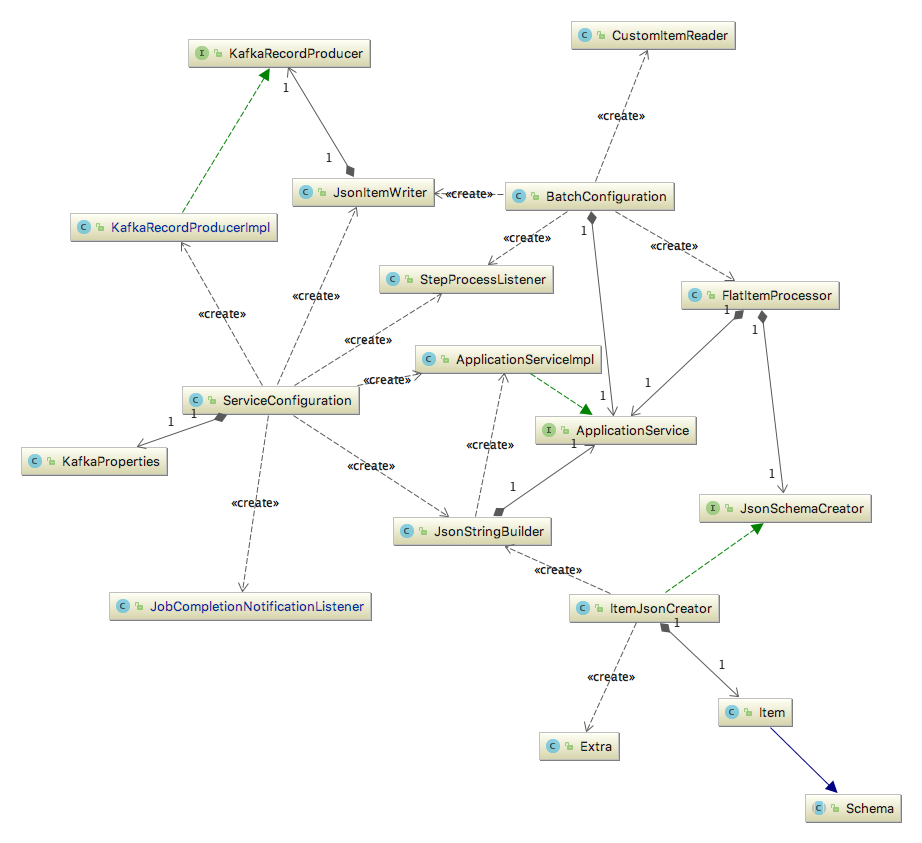
\includegraphics[width=1.00\textwidth]{images/domain_model.png}
	\caption{Relation of classes of a Simple Flat File Importer}%
	\label{fig:importer-classes-relations}%
\end{figure}


Figure \ref{fig:importer-classes-relations} shows a more detailed view of classes inside a simple flat file importer and how they are related together.

\subsection{Framework Features}\label{framework-features}

\begin{itemize}
\tightlist
\item
  Ability to import data with various types and formats
\item
  A Module with pre-packaged utility classes

  \begin{itemize}
  \tightlist
  \item
    Just import and ready to use utility classes
  \end{itemize}
\item
  Independent Cloud Tasks as microservices
\item
  Logging and tracing execution of jobs in different steps
\end{itemize}

\subsection{Framework Strengths}\label{framework-strengths}

\begin{itemize}
\tightlist
\item
  Usability

  \begin{itemize}
  \tightlist
  \item
    Reusable, ready-to-use functionalities
  \end{itemize}
\item
  Extensibility

  \begin{itemize}
  \tightlist
  \item
    Ability to add custom utilities
  \item
    Easy to add new jobs
  \end{itemize}
\item
  Portability

  \begin{itemize}
  \tightlist
  \item
    Jobs run as microservices
  \item
    Every importer could be packed into JAR file and deployed into
    private or public cloud
  \end{itemize}
\end{itemize}

\subsection{Supported Data Formats}\label{supported-data-formats}

The sources which we used have come in various types and formats.
Therefore different data formats and types have been implemented for
importing through our framework such as: - REST Interface, HTTP and FTP
data source types - Delimiter-separated value (DSV) - CSV - TSV - HTML -
XLS - XLXS

\subsection{Possible Further
Improvements}\label{possible-further-improvements}

\begin{enumerate}
\def\labelenumi{\arabic{enumi}.}
\tightlist
\item
  Scheduling jobs for every importer within the Framework: until now,
  the scheduling of importing jobs is done by Kubernetes, but this
  functionality could be provided by Spring via an embeddable component
  such as (Quartz). This feature would easily allow the scheduling of
  jobs at specific times.
\item
  Recoverability of jobs from failures: Currently the intermediate
  results of job processing are stored in an in-memory database (H2)
  inside the importer. As we containerized every importer into Docker
  containers, this functionality will disappear when the container
  terminates. The solution would be to create and configure a single
  relational database to store all the intermediary results of the jobs
  executions; whenever an importer crashes and is restarted, it will
  start from the last point that it stopped.
\end{enumerate}

\subsection{The Values of the
Framework}\label{the-values-of-the-framework}

\begin{itemize}
\tightlist
\item
  The application of our already built framework is mostly required for
  huge data integration and migration.
\item
  Useful functionalities are ready to use just by importing them.
\item
  It is very easy to extend it by adding new data sources to import and
  some new functions such as unit conversions.
\item
  Writing transformed data to the pipeline (i.e.~the queue) is
  abstracted away from the user and provided by the framework.
\item
  Well defined, clean code with clear comments.
\end{itemize}
